\documentclass[11pt,preprint, authoryear]{elsarticle}

\usepackage{lmodern}
%%%% My spacing
\usepackage{setspace}
\setstretch{1.2}
\DeclareMathSizes{12}{14}{10}{10}

% Wrap around which gives all figures included the [H] command, or places it "here". This can be tedious to code in Rmarkdown.
\usepackage{float}
\let\origfigure\figure
\let\endorigfigure\endfigure
\renewenvironment{figure}[1][2] {
    \expandafter\origfigure\expandafter[H]
} {
    \endorigfigure
}

\let\origtable\table
\let\endorigtable\endtable
\renewenvironment{table}[1][2] {
    \expandafter\origtable\expandafter[H]
} {
    \endorigtable
}


\usepackage{ifxetex,ifluatex}
\usepackage{fixltx2e} % provides \textsubscript
\ifnum 0\ifxetex 1\fi\ifluatex 1\fi=0 % if pdftex
  \usepackage[T1]{fontenc}
  \usepackage[utf8]{inputenc}
\else % if luatex or xelatex
  \ifxetex
    \usepackage{mathspec}
    \usepackage{xltxtra,xunicode}
  \else
    \usepackage{fontspec}
  \fi
  \defaultfontfeatures{Mapping=tex-text,Scale=MatchLowercase}
  \newcommand{\euro}{€}
\fi

\usepackage{amssymb, amsmath, amsthm, amsfonts}

\def\bibsection{\section*{References}} %%% Make "References" appear before bibliography


\usepackage[round]{natbib}

\usepackage{longtable}
\usepackage[margin=2.3cm,bottom=2cm,top=2.5cm, includefoot]{geometry}
\usepackage{fancyhdr}
\usepackage[bottom, hang, flushmargin]{footmisc}
\usepackage{graphicx}
\numberwithin{equation}{section}
\numberwithin{figure}{section}
\numberwithin{table}{section}
\setlength{\parindent}{0cm}
\setlength{\parskip}{1.3ex plus 0.5ex minus 0.3ex}
\usepackage{textcomp}
\renewcommand{\headrulewidth}{0.2pt}
\renewcommand{\footrulewidth}{0.3pt}

\usepackage{array}
\newcolumntype{x}[1]{>{\centering\arraybackslash\hspace{0pt}}p{#1}}

%%%%  Remove the "preprint submitted to" part. Don't worry about this either, it just looks better without it:
\makeatletter
\def\ps@pprintTitle{%
  \let\@oddhead\@empty
  \let\@evenhead\@empty
  \let\@oddfoot\@empty
  \let\@evenfoot\@oddfoot
}
\makeatother

 \def\tightlist{} % This allows for subbullets!

\usepackage{hyperref}
\hypersetup{breaklinks=true,
            bookmarks=true,
            colorlinks=true,
            citecolor=blue,
            urlcolor=blue,
            linkcolor=blue,
            pdfborder={0 0 0}}


% The following packages allow huxtable to work:
\usepackage{siunitx}
\usepackage{multirow}
\usepackage{hhline}
\usepackage{calc}
\usepackage{tabularx}
\usepackage{booktabs}
\usepackage{caption}


\newenvironment{columns}[1][]{}{}

\newenvironment{column}[1]{\begin{minipage}{#1}\ignorespaces}{%
\end{minipage}
\ifhmode\unskip\fi
\aftergroup\useignorespacesandallpars}

\def\useignorespacesandallpars#1\ignorespaces\fi{%
#1\fi\ignorespacesandallpars}

\makeatletter
\def\ignorespacesandallpars{%
  \@ifnextchar\par
    {\expandafter\ignorespacesandallpars\@gobble}%
    {}%
}
\makeatother

\newlength{\cslhangindent}
\setlength{\cslhangindent}{1.5em}
\newenvironment{CSLReferences}%
  {\setlength{\parindent}{0pt}%
  \everypar{\setlength{\hangindent}{\cslhangindent}}\ignorespaces}%
  {\par}


\urlstyle{same}  % don't use monospace font for urls
\setlength{\parindent}{0pt}
\setlength{\parskip}{6pt plus 2pt minus 1pt}
\setlength{\emergencystretch}{3em}  % prevent overfull lines
\setcounter{secnumdepth}{5}

%%% Use protect on footnotes to avoid problems with footnotes in titles
\let\rmarkdownfootnote\footnote%
\def\footnote{\protect\rmarkdownfootnote}
\IfFileExists{upquote.sty}{\usepackage{upquote}}{}

%%% Include extra packages specified by user
\usepackage{booktabs}
\usepackage{longtable}
\usepackage{array}
\usepackage{multirow}
\usepackage{wrapfig}
\usepackage{float}
\usepackage{colortbl}
\usepackage{pdflscape}
\usepackage{tabu}
\usepackage{threeparttable}
\usepackage{threeparttablex}
\usepackage[normalem]{ulem}
\usepackage{makecell}
\usepackage{xcolor}
\usepackage{caption}
\usepackage{graphicx}
\usepackage{siunitx}
\usepackage{hhline}
\usepackage{calc}
\usepackage{tabularx}
\usepackage{adjustbox}
\usepackage{hyperref}

%%% Hard setting column skips for reports - this ensures greater consistency and control over the length settings in the document.
%% page layout
%% paragraphs
\setlength{\baselineskip}{12pt plus 0pt minus 0pt}
\setlength{\parskip}{12pt plus 0pt minus 0pt}
\setlength{\parindent}{0pt plus 0pt minus 0pt}
%% floats
\setlength{\floatsep}{12pt plus 0 pt minus 0pt}
\setlength{\textfloatsep}{20pt plus 0pt minus 0pt}
\setlength{\intextsep}{14pt plus 0pt minus 0pt}
\setlength{\dbltextfloatsep}{20pt plus 0pt minus 0pt}
\setlength{\dblfloatsep}{14pt plus 0pt minus 0pt}
%% maths
\setlength{\abovedisplayskip}{12pt plus 0pt minus 0pt}
\setlength{\belowdisplayskip}{12pt plus 0pt minus 0pt}
%% lists
\setlength{\topsep}{10pt plus 0pt minus 0pt}
\setlength{\partopsep}{3pt plus 0pt minus 0pt}
\setlength{\itemsep}{5pt plus 0pt minus 0pt}
\setlength{\labelsep}{8mm plus 0mm minus 0mm}
\setlength{\parsep}{\the\parskip}
\setlength{\listparindent}{\the\parindent}
%% verbatim
\setlength{\fboxsep}{5pt plus 0pt minus 0pt}



\begin{document}



%titlepage
\thispagestyle{empty}
\begin{center}
\begin{minipage}{0.75\linewidth}
    \centering
%Entry1
    {\uppercase{\huge LATE to the Party: Investigating Instrument
Variables for Education\par}}
    \vspace{2cm}
%Author's name
    {\LARGE \textbf{Cassandra Pengelly}\par}
    \vspace{1cm}
%University logo
\begin{center}
    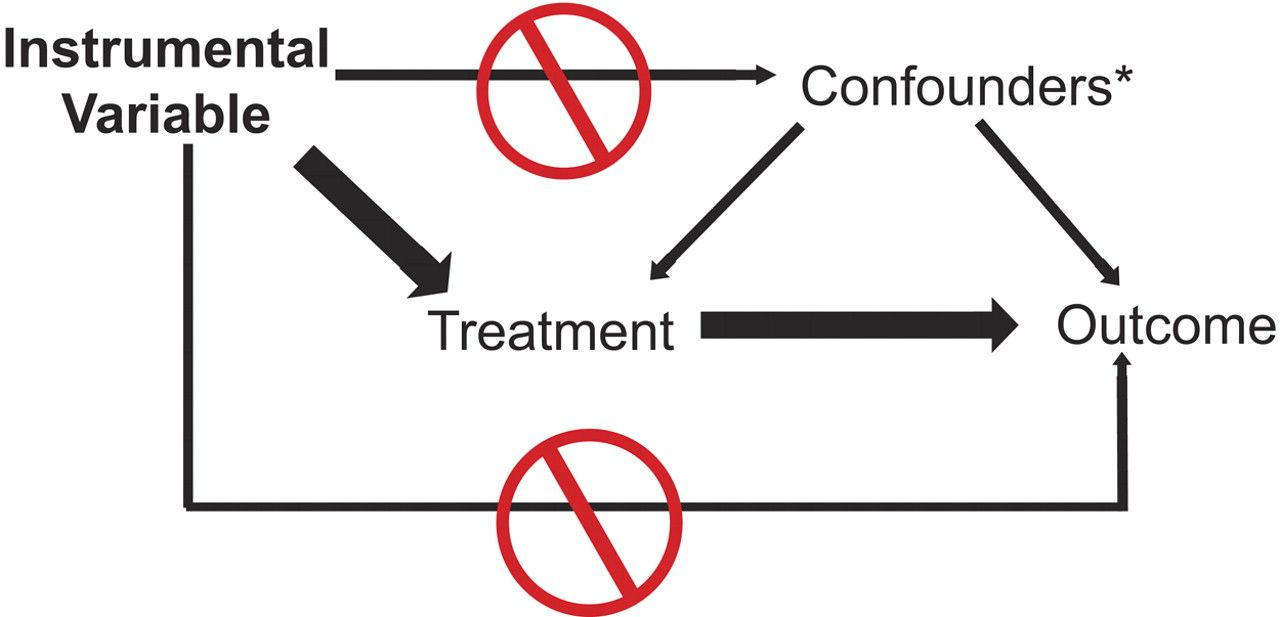
\includegraphics[width=1\linewidth]{Tex/logo.jpeg}
\end{center}
\vspace{1cm}
%Supervisor's Details
\begin{center}
    {\Large 20346212\par}
    \vspace{1cm}
%Degree
    {\large \textbf{Econometrics 871: Cross Section Project}\par}
    \vspace{1cm}
%Institution
    {\large Stellenbosch University\par}
    \vspace{1cm}
%Date
    {\large July 2021}
%More
    {\normalsize }
%More
    {\normalsize }
\end{center}
\end{minipage}
\end{center}
\clearpage


\begin{frontmatter}  %

\title{}

% Set to FALSE if wanting to remove title (for submission)


\vspace{1cm}





\vspace{0.5cm}

\end{frontmatter}


\renewcommand{\contentsname}{Table of Contents}
{\tableofcontents}

%________________________
% Header and Footers
%%%%%%%%%%%%%%%%%%%%%%%%%%%%%%%%%
\pagestyle{fancy}
\chead{}
\rhead{}
\lfoot{}
\rfoot{\footnotesize Page \thepage}
\lhead{}
%\rfoot{\footnotesize Page \thepage } % "e.g. Page 2"
\cfoot{}

%\setlength\headheight{30pt}
%%%%%%%%%%%%%%%%%%%%%%%%%%%%%%%%%
%________________________

\headsep 35pt % So that header does not go over title




\newpage

\hypertarget{introduction}{%
\section{\texorpdfstring{Introduction
\label{Introduction}}{Introduction }}\label{introduction}}

The return to education is a cornerstone topic in labour economics and
is of particular interest to policymakers. This is no different in South
Africa, especially given the significant income inequality, which is
often claimed to be strongly linked to differences in education.
However, wages cannot simply be regressed on education because there is
likely endogeneity present. This arises from the problem of there being
an omitted variable, where education and wages are both correlated with
a variable in the error term. One variable of this nature that has been
extensively studied is innate ability
(\protect\hyperlink{ref-hertz}{Hertz}
(\protect\hyperlink{ref-hertz}{2003})). Returns to schooling could be
biased upwards if ability is positively correlated with both income and
education. However, as \protect\hyperlink{ref-disc}{Lang}
(\protect\hyperlink{ref-disc}{1993}) assesses, the overall findings of
research on the impact of ability bias are inconclusive. In fact,
\protect\hyperlink{ref-disc}{Lang} (\protect\hyperlink{ref-disc}{1993:
1}) notes that several papers find that returns to education are
\emph{downwardly} biased.

This paper will investigate whether OLS estimates are biased in the
South African case by estimating the return to education using four
different instrumental variable estimators: the first two exploit
parents' education, and the other two use parents' occupations. These
instruments estimate a `local average treatment effect', which - this
paper will argue - is more appropriate than OLS estimators for analysing
the returns to education for South Africa. These instruments are tested
for strength and validity and then implemented on the NIDS Wave 5 data
set. This essay\footnote{This essay was written in R using the Texevier
  package by \protect\hyperlink{ref-Texevier}{Katzke}
  (\protect\hyperlink{ref-Texevier}{2017})} is structured as follows:
section \ref{data} details the data set used and discusses the
descriptive statistics. Section \ref{meth} outlines the methodology and
argues that the LATE assumptions for the instrumental variables hold.
Following this, section \ref{results} presents the regression results
and evaluates the robustness of the estimators used to obtain a causal
effect. The final section, \ref{conclusion}, concludes\footnote{The code
  and write up for this project can be found on Github
  \url{https://github.com/cass-code/Cross-Section.git}}.

\hypertarget{data}{%
\section{\texorpdfstring{Data \label{data}}{Data }}\label{data}}

The data used for this paper is sourced from the National Income
Dynamics Survey (NIDS) (\protect\hyperlink{ref-nids}{\emph{National
income dynamics study 2017, wave 5 dataset}}
(\protect\hyperlink{ref-nids}{2018})), which was the first national
household panel study in South Africa. NIDS is an initiative of the
Department of Planning, Monitoring and Evaluation, and the Southern
Africa Labour and Development Research Unit (SALDRU) is tasked with
implementation (\protect\hyperlink{ref-nids5}{Brophy, Branson, Daniels,
Leibbrandt, Mlatsheni \& Woolard}
(\protect\hyperlink{ref-nids5}{2018})). NIDS was started in 2008,
interviewing over 28,000 people. These same people are then interviewed
every two years. The latest survey is Wave 5 (2017), which is the data
set used for the regression analysis, where the individual is the unit
of observation. Wave 5 consists of 37,368 individuals, where the high
rate of attrition among high-income, Indian/Asian, and White respondents
has led to the sample being increased by 2,775 to maintain sample
representativeness (\protect\hyperlink{ref-nids5}{Brophy, Branson,
Daniels, Leibbrandt, Mlatsheni \& Woolard}
(\protect\hyperlink{ref-nids5}{2018})).

\protect\hyperlink{ref-nids1}{Villiers, Leibbrandt \& Woolard}
(\protect\hyperlink{ref-nids1}{2009}) outlays the design of the survey.
To sample the households used in Wave 1, two-stage cluster sample design
with stratification was employed. Stage 1 involved selecting 400 Primary
Sampling Units, based on Statistics South Africa's Master Sample of 300
Primary Sampling Units (2003). Private households in all of South
Africa's 9 provinces are the target population for NIDS. The 53
disctrict councils make up the explicit strata in the Master sample.
Based on the allocation of the district councils in the Primary Sampling
Units in the Master Sample, the sample was proportionally allocated and
the Primary Sampling Units were randomly chosen within the strata
(\protect\hyperlink{ref-nids1}{Villiers, Leibbrandt \& Woolard}
(\protect\hyperlink{ref-nids1}{2009}) p.9). Fieldworkers are assigned to
the selected addresses and are instructed to interview all households
living at the dwelling unit.

The NIDS wave 5 data set contains 30,110 observations of 1,144
variables. As a part of the data cleaning process, I selected 14
variables: year of birth, gender, race, income, marital status, highest
level of schooling, highest level of tertiary education, union status,
father's schooling, father's tertiary education, father's occupation,
mother's schooling, mother's tertiary education, and mother's
occupation. The occupation variables have been re-coded with the
appropriate profession names from the
\protect\hyperlink{ref-isco}{\emph{International standard classification
of occupations}} (\protect\hyperlink{ref-isco}{2012}), and are therefore
categorical variables. I constructed the variables age and age-squared
from the year of birth, and I constructed an education variable, which
represents the number of years of education for an individual
(i.e.~summing the years of schooling and years of tertiary education). I
constructed a similar variable for mother and father's education.
Unfortunately, there are a significant number of missing observations
for the variables income, parents' education, marital status and union
status. Because of this, the sample size for the regressions is reduced
to 3,300 and under.

As a part of the initial data exploration, figure \ref{Figure1} gives a
quick snapshot of the relationship between income and education. As
shown by the black regression line, income and education are positively
correlated, which is what we expect. Section \ref{results} will argue
that this is a causal relationship. We can also glimpse how education
and income is distributed in the sample. To get a clearer view of the
race distribution, figure \ref{Figure2} shows a bar plot of the four
main race groups in South Africa: African, Asian/Indian, Coloured and
White. The graph shows the sample is roughly representative of the South
African population, with a slightly smaller sample of Coloured and White
individuals (despite the top up sample). We also want to check that
income is normally distributed to combat heteroskedasticity in the
regression analysis. We find that the income distribution is skewed but
log of income is fairly normal, as figure \ref{Figure3} shows. This
indicates that log of income should be the dependent variable in the
regressions (rather the linear form of income), which is also supported
by the literature.

\begin{figure}[H]

{\centering \includegraphics{20346212CSproj_files/figure-latex/lineargraph-1} 

}

\caption{Income and Education Relationship \label{Figure1}}\label{fig:lineargraph}
\end{figure}

\begin{figure}[H]

{\centering \includegraphics{20346212CSproj_files/figure-latex/racegraph-1} 

}

\caption{Race Proportions of Sample \label{Figure2}}\label{fig:racegraph}
\end{figure}

\begin{figure}[H]

{\centering \includegraphics{20346212CSproj_files/figure-latex/incomergraph-1} 

}

\caption{Log Income Distribution  \label{Figure3}}\label{fig:incomergraph}
\end{figure}

\hypertarget{methodology}{%
\section{\texorpdfstring{Methodology
\label{meth}}{Methodology }}\label{methodology}}

Following the earnings function proposed by
\protect\hyperlink{ref-mince}{Mincer}
(\protect\hyperlink{ref-mince}{1974}), to model the relationship between
income and education in \ref{reg1}, the following general OLS
regression, \ref{eq1}, is used: \begin{align}
Log(income)=\beta_{0}+\beta_{1} X_{1}+\cdots+\beta_{k} X_{k}+u  \label{eq1}
\end{align} where \(X_{1}\) is education and \(\ldots, X_{k}\) includes
the other regressors: age, age-squared, race and gender,
\(\beta_{0}, \ldots, \beta_{k}\) are the regression coefficients, and
\(u\) is the error term. Race is a categorical variable with the
reference group as African, and gender is a dummy variable that takes a
value of 1 if an individual is male and 0 otherwise.

If education is an endogenous regressor - i.e.~correlated with the error
term - then the OLS coefficient for education (\(\beta_{1}\)) will be
biased (\protect\hyperlink{ref-R}{Colonescu}
(\protect\hyperlink{ref-R}{2016})). If we can find an instrumental
variable for education, then we can remove this endogeneity and get an
unbiased coefficient for education
(\protect\hyperlink{ref-metrics}{Stock \& Watson}
(\protect\hyperlink{ref-metrics}{2015}) \&
\protect\hyperlink{ref-metrics1}{Venables \& Smith}
(\protect\hyperlink{ref-metrics1}{2010})). 4 different variables are
used as an instrument for an individual's education: fathers education,
mother's education, father's occupation and mother's occupation. In
order to use these variables as instruments, we have to check their
validity(\protect\hyperlink{ref-ang}{Imbens \& Angrist}
(\protect\hyperlink{ref-ang}{1994})). Economic theory and the literature
suggests that returns to schooling are heterogeneous
(\protect\hyperlink{ref-return}{Koop \& Tobias}
(\protect\hyperlink{ref-return}{2004: 827--828})), which implies that
for the instruments to be valid they have to comply with the Local
Average Treatment Effects (LATE) identifying assumptions. The four LATE
assumptions are: independence, random assignment, exclusion restriction,
and monotonicity. The first section below, ref\{spec\}, interprets the
diagnostic tests for instrument variables and the second part,
ref\{late\}, evaluates whether the LATE assumptions hold for the
instrument variables.

\hypertarget{specification-tests}{%
\subsection{\texorpdfstring{Specification Tests
\label{spec}}{Specification Tests }}\label{specification-tests}}

\begin{table}

\caption{\label{tab:Specification}Specification Tests for Father's Education \label{FE}}
\centering
\begin{tabular}[t]{l|r|r|r|r}
\hline
  & df1 & df2 & statistic & p-value\\
\hline
Weak instruments & 1 & 3368 & 406.13620 & 0\\
\hline
Wu-Hausman & 1 & 3367 & 70.06385 & 0\\
\hline
Sargan & 0 & NA & NA & NA\\
\hline
\end{tabular}
\end{table}

\begin{table}

\caption{\label{tab:Specification}Specification Tests for Mother's Education \label{ME}}
\centering
\begin{tabular}[t]{l|r|r|r|r}
\hline
  & df1 & df2 & statistic & p-value\\
\hline
Weak instruments & 1 & 3605 & 400.15525 & 0\\
\hline
Wu-Hausman & 1 & 3604 & 46.19299 & 0\\
\hline
Sargan & 0 & NA & NA & NA\\
\hline
\end{tabular}
\end{table}

\begin{table}

\caption{\label{tab:Specification}Specification Tests for Father's Occupation \label{FO}}
\centering
\begin{tabular}[t]{l|r|r|r|r}
\hline
  & df1 & df2 & statistic & p-value\\
\hline
Weak instruments & 9 & 2162 & 19.86956 & 0.0000000\\
\hline
Wu-Hausman & 1 & 2169 & 32.61388 & 0.0000000\\
\hline
Sargan & 8 & NA & 12.65711 & 0.1242046\\
\hline
\end{tabular}
\end{table}

\begin{table}

\caption{\label{tab:Specification}Specification Tests for Mother's Occupation \label{MO}}
\centering
\begin{tabular}[t]{l|r|r|r|r}
\hline
  & df1 & df2 & statistic & p-value\\
\hline
Weak instruments & 9 & 1731 & 38.61704 & 0.000000\\
\hline
Wu-Hausman & 1 & 1738 & 64.04297 & 0.000000\\
\hline
Sargan & 8 & NA & 4.50194 & 0.809239\\
\hline
\end{tabular}
\end{table}

\hypertarget{late-assumptions}{%
\subsection{\texorpdfstring{LATE Assumptions
\label{late}}{LATE Assumptions }}\label{late-assumptions}}

If our instrument is: 1. randomly assigned 2. only affects our outcome
through its effect on our endogenous variable 3. has a significant
impact on take-up of treatment, and 4. does not deter anyone from
treatment

Random Assignment: Random assignment of draft eligibility means
independence assumption is very convincing. Would not expect individuals
who were born on low-lottery days to have different potential earnings
distributions or potential take-up probabilities than high-lottery
individuals.

Exclusion restriction: More reason to be concerned. Draft eligible men
were allowed to defer their military service if they wanted to proceed
with their studies. If some men decided to get more schooling because
they had low lottery numbers and did not want to serve in the military,
then this could have affected earnings via education attainment rather
than via military service.

Monotonicity: It seemse unlikely that someone who would have pursued
education further would decide not to because either of his/her parent
pursued education further. Thus, it's reasonable to conclude that the
monotonicity assumption holds (i.e.~there are no defiers). Similarly

Is it possible that someone would have volunteered for the army (if
draft ineligible) but decided not to because of draft eligibility? Seems
unlikely.

The relevance assumption is testable and table ref\{reg5\} shows that
both parents' education is correlated with education (and the
coefficients are statistically significant at a 1\% level). This means
these instruments affect treatment for at least some individuals. The
regression of education on parents' occupation shows that joint effect
of the occupation types are significant. The p-values associated with
the F-test for each regression are presented in \ref{tab}. The p-values
are essentially 0 and thus reject the null hypothesis that the joint
effect is zero. From an intuitive stand point, if an individual's
parents pursued more years of education,

Are there individuals who would not have gone to war if they didn't get
picked, but ended up going just because they were eligible? Seems
plausible.

 
  \providecommand{\huxb}[2]{\arrayrulecolor[RGB]{#1}\global\arrayrulewidth=#2pt}
  \providecommand{\huxvb}[2]{\color[RGB]{#1}\vrule width #2pt}
  \providecommand{\huxtpad}[1]{\rule{0pt}{#1}}
  \providecommand{\huxbpad}[1]{\rule[-#1]{0pt}{#1}}

\begin{table}[ht]
\begin{centerbox}
\begin{threeparttable}
\captionsetup{justification=centering,singlelinecheck=off}
\caption{Regressions: Instrument Relevance}
 \label{reg5}
\setlength{\tabcolsep}{0pt}
\begin{tabular}{l l l}


\hhline{>{\huxb{0, 0, 0}{0.8}}->{\huxb{0, 0, 0}{0.8}}->{\huxb{0, 0, 0}{0.8}}-}
\arrayrulecolor{black}

\multicolumn{1}{!{\huxvb{0, 0, 0}{0}}c!{\huxvb{0, 0, 0}{0}}}{\huxtpad{6pt + 1em}\centering \hspace{6pt} {\fontsize{11pt}{13.2pt}\selectfont } \hspace{6pt}\huxbpad{6pt}} &
\multicolumn{1}{c!{\huxvb{0, 0, 0}{0}}}{\huxtpad{6pt + 1em}\centering \hspace{6pt} {\fontsize{11pt}{13.2pt}\selectfont Education} \hspace{6pt}\huxbpad{6pt}} &
\multicolumn{1}{c!{\huxvb{0, 0, 0}{0}}}{\huxtpad{6pt + 1em}\centering \hspace{6pt} {\fontsize{11pt}{13.2pt}\selectfont Education} \hspace{6pt}\huxbpad{6pt}} \tabularnewline[-0.5pt]


\hhline{>{\huxb{255, 255, 255}{0.4}}->{\huxb{0, 0, 0}{0.4}}->{\huxb{0, 0, 0}{0.4}}-}
\arrayrulecolor{black}

\multicolumn{1}{!{\huxvb{0, 0, 0}{0}}l!{\huxvb{0, 0, 0}{0}}}{\huxtpad{6pt + 1em}\raggedright \hspace{6pt} {\fontsize{11pt}{13.2pt}\selectfont Father's Education} \hspace{6pt}\huxbpad{6pt}} &
\multicolumn{1}{r!{\huxvb{0, 0, 0}{0}}}{\huxtpad{6pt + 1em}\raggedleft \hspace{6pt} {\fontsize{11pt}{13.2pt}\selectfont 0.234 ***} \hspace{6pt}\huxbpad{6pt}} &
\multicolumn{1}{r!{\huxvb{0, 0, 0}{0}}}{\huxtpad{6pt + 1em}\raggedleft \hspace{6pt} {\fontsize{11pt}{13.2pt}\selectfont ~~~~~~~~} \hspace{6pt}\huxbpad{6pt}} \tabularnewline[-0.5pt]


\hhline{}
\arrayrulecolor{black}

\multicolumn{1}{!{\huxvb{0, 0, 0}{0}}l!{\huxvb{0, 0, 0}{0}}}{\huxtpad{6pt + 1em}\raggedright \hspace{6pt} {\fontsize{11pt}{13.2pt}\selectfont } \hspace{6pt}\huxbpad{6pt}} &
\multicolumn{1}{r!{\huxvb{0, 0, 0}{0}}}{\huxtpad{6pt + 1em}\raggedleft \hspace{6pt} {\fontsize{11pt}{13.2pt}\selectfont (0.008)~~~} \hspace{6pt}\huxbpad{6pt}} &
\multicolumn{1}{r!{\huxvb{0, 0, 0}{0}}}{\huxtpad{6pt + 1em}\raggedleft \hspace{6pt} {\fontsize{11pt}{13.2pt}\selectfont ~~~~~~~~} \hspace{6pt}\huxbpad{6pt}} \tabularnewline[-0.5pt]


\hhline{}
\arrayrulecolor{black}

\multicolumn{1}{!{\huxvb{0, 0, 0}{0}}l!{\huxvb{0, 0, 0}{0}}}{\huxtpad{6pt + 1em}\raggedright \hspace{6pt} {\fontsize{11pt}{13.2pt}\selectfont Mother's Education} \hspace{6pt}\huxbpad{6pt}} &
\multicolumn{1}{r!{\huxvb{0, 0, 0}{0}}}{\huxtpad{6pt + 1em}\raggedleft \hspace{6pt} {\fontsize{11pt}{13.2pt}\selectfont ~~~~~~~~} \hspace{6pt}\huxbpad{6pt}} &
\multicolumn{1}{r!{\huxvb{0, 0, 0}{0}}}{\huxtpad{6pt + 1em}\raggedleft \hspace{6pt} {\fontsize{11pt}{13.2pt}\selectfont 0.247 ***} \hspace{6pt}\huxbpad{6pt}} \tabularnewline[-0.5pt]


\hhline{}
\arrayrulecolor{black}

\multicolumn{1}{!{\huxvb{0, 0, 0}{0}}l!{\huxvb{0, 0, 0}{0}}}{\huxtpad{6pt + 1em}\raggedright \hspace{6pt} {\fontsize{11pt}{13.2pt}\selectfont } \hspace{6pt}\huxbpad{6pt}} &
\multicolumn{1}{r!{\huxvb{0, 0, 0}{0}}}{\huxtpad{6pt + 1em}\raggedleft \hspace{6pt} {\fontsize{11pt}{13.2pt}\selectfont ~~~~~~~~} \hspace{6pt}\huxbpad{6pt}} &
\multicolumn{1}{r!{\huxvb{0, 0, 0}{0}}}{\huxtpad{6pt + 1em}\raggedleft \hspace{6pt} {\fontsize{11pt}{13.2pt}\selectfont (0.008)~~~} \hspace{6pt}\huxbpad{6pt}} \tabularnewline[-0.5pt]


\hhline{>{\huxb{255, 255, 255}{0.4}}->{\huxb{0, 0, 0}{0.4}}->{\huxb{0, 0, 0}{0.4}}-}
\arrayrulecolor{black}

\multicolumn{1}{!{\huxvb{0, 0, 0}{0}}l!{\huxvb{0, 0, 0}{0}}}{\huxtpad{6pt + 1em}\raggedright \hspace{6pt} {\fontsize{11pt}{13.2pt}\selectfont N} \hspace{6pt}\huxbpad{6pt}} &
\multicolumn{1}{r!{\huxvb{0, 0, 0}{0}}}{\huxtpad{6pt + 1em}\raggedleft \hspace{6pt} {\fontsize{11pt}{13.2pt}\selectfont 3376~~~~~~~~} \hspace{6pt}\huxbpad{6pt}} &
\multicolumn{1}{r!{\huxvb{0, 0, 0}{0}}}{\huxtpad{6pt + 1em}\raggedleft \hspace{6pt} {\fontsize{11pt}{13.2pt}\selectfont 3613~~~~~~~~} \hspace{6pt}\huxbpad{6pt}} \tabularnewline[-0.5pt]


\hhline{}
\arrayrulecolor{black}

\multicolumn{1}{!{\huxvb{0, 0, 0}{0}}l!{\huxvb{0, 0, 0}{0}}}{\huxtpad{6pt + 1em}\raggedright \hspace{6pt} {\fontsize{11pt}{13.2pt}\selectfont R2} \hspace{6pt}\huxbpad{6pt}} &
\multicolumn{1}{r!{\huxvb{0, 0, 0}{0}}}{\huxtpad{6pt + 1em}\raggedleft \hspace{6pt} {\fontsize{11pt}{13.2pt}\selectfont 0.190~~~~} \hspace{6pt}\huxbpad{6pt}} &
\multicolumn{1}{r!{\huxvb{0, 0, 0}{0}}}{\huxtpad{6pt + 1em}\raggedleft \hspace{6pt} {\fontsize{11pt}{13.2pt}\selectfont 0.197~~~~} \hspace{6pt}\huxbpad{6pt}} \tabularnewline[-0.5pt]


\hhline{>{\huxb{0, 0, 0}{0.8}}->{\huxb{0, 0, 0}{0.8}}->{\huxb{0, 0, 0}{0.8}}-}
\arrayrulecolor{black}

\multicolumn{3}{!{\huxvb{0, 0, 0}{0}}l!{\huxvb{0, 0, 0}{0}}}{\huxtpad{6pt + 1em}\raggedright \hspace{6pt} {\fontsize{11pt}{13.2pt}\selectfont  *** p $<$ 0.001;  ** p $<$ 0.01;  * p $<$ 0.05.} \hspace{6pt}\huxbpad{6pt}} \tabularnewline[-0.5pt]


\hhline{}
\arrayrulecolor{black}
\end{tabular}
\end{threeparttable}\par\end{centerbox}

\end{table}
 

\begin{table}

\caption{\label{tab:unnamed-chunk-1}p-values of F statistics \label{tab}}
\centering
\begin{tabular}[t]{l|l}
\hline
Regression & p.value\\
\hline
Regress Education on Father's Occupation & 4.748773e-54\\
\hline
Regress Education on Mother's Occupation & 2.356427e-61\\
\hline
\end{tabular}
\end{table}

\hypertarget{results}{%
\section{\texorpdfstring{Results
\label{results}}{Results }}\label{results}}

Table \ref{reg1} presents the regressions results and figure \ref{plot}
plots the regression coefficients with their 95\% confidence intervals.

 
  \providecommand{\huxb}[2]{\arrayrulecolor[RGB]{#1}\global\arrayrulewidth=#2pt}
  \providecommand{\huxvb}[2]{\color[RGB]{#1}\vrule width #2pt}
  \providecommand{\huxtpad}[1]{\rule{0pt}{#1}}
  \providecommand{\huxbpad}[1]{\rule[-#1]{0pt}{#1}}

\begin{table}[ht]
\begin{centerbox}
\begin{threeparttable}
\captionsetup{justification=centering,singlelinecheck=off}
\caption{Regressions: OLS and 2SLS with Various Instruments}
 \label{reg1}
\setlength{\tabcolsep}{0pt}
\begin{tabular}{l l l l l l}


\hhline{>{\huxb{0, 0, 0}{0.8}}->{\huxb{0, 0, 0}{0.8}}->{\huxb{0, 0, 0}{0.8}}->{\huxb{0, 0, 0}{0.8}}->{\huxb{0, 0, 0}{0.8}}->{\huxb{0, 0, 0}{0.8}}-}
\arrayrulecolor{black}

\multicolumn{1}{!{\huxvb{0, 0, 0}{0}}c!{\huxvb{0, 0, 0}{0}}}{\huxtpad{6pt + 1em}\centering \hspace{6pt} {\fontsize{11pt}{13.2pt}\selectfont } \hspace{6pt}\huxbpad{6pt}} &
\multicolumn{1}{c!{\huxvb{0, 0, 0}{0}}}{\huxtpad{6pt + 1em}\centering \hspace{6pt} {\fontsize{11pt}{13.2pt}\selectfont OLS} \hspace{6pt}\huxbpad{6pt}} &
\multicolumn{1}{c!{\huxvb{0, 0, 0}{0}}}{\huxtpad{6pt + 1em}\centering \hspace{6pt} {\fontsize{11pt}{13.2pt}\selectfont 2SLS FE} \hspace{6pt}\huxbpad{6pt}} &
\multicolumn{1}{c!{\huxvb{0, 0, 0}{0}}}{\huxtpad{6pt + 1em}\centering \hspace{6pt} {\fontsize{11pt}{13.2pt}\selectfont 2SLS ME} \hspace{6pt}\huxbpad{6pt}} &
\multicolumn{1}{c!{\huxvb{0, 0, 0}{0}}}{\huxtpad{6pt + 1em}\centering \hspace{6pt} {\fontsize{11pt}{13.2pt}\selectfont 2SLS FO} \hspace{6pt}\huxbpad{6pt}} &
\multicolumn{1}{c!{\huxvb{0, 0, 0}{0}}}{\huxtpad{6pt + 1em}\centering \hspace{6pt} {\fontsize{11pt}{13.2pt}\selectfont 2SLS MO} \hspace{6pt}\huxbpad{6pt}} \tabularnewline[-0.5pt]


\hhline{>{\huxb{255, 255, 255}{0.4}}->{\huxb{0, 0, 0}{0.4}}->{\huxb{0, 0, 0}{0.4}}->{\huxb{0, 0, 0}{0.4}}->{\huxb{0, 0, 0}{0.4}}->{\huxb{0, 0, 0}{0.4}}-}
\arrayrulecolor{black}

\multicolumn{1}{!{\huxvb{0, 0, 0}{0}}l!{\huxvb{0, 0, 0}{0}}}{\huxtpad{6pt + 1em}\raggedright \hspace{6pt} {\fontsize{11pt}{13.2pt}\selectfont Age} \hspace{6pt}\huxbpad{6pt}} &
\multicolumn{1}{r!{\huxvb{0, 0, 0}{0}}}{\huxtpad{6pt + 1em}\raggedleft \hspace{6pt} {\fontsize{11pt}{13.2pt}\selectfont 0.047 ***} \hspace{6pt}\huxbpad{6pt}} &
\multicolumn{1}{r!{\huxvb{0, 0, 0}{0}}}{\huxtpad{6pt + 1em}\raggedleft \hspace{6pt} {\fontsize{11pt}{13.2pt}\selectfont 0.040 ***} \hspace{6pt}\huxbpad{6pt}} &
\multicolumn{1}{r!{\huxvb{0, 0, 0}{0}}}{\huxtpad{6pt + 1em}\raggedleft \hspace{6pt} {\fontsize{11pt}{13.2pt}\selectfont 0.049 ***} \hspace{6pt}\huxbpad{6pt}} &
\multicolumn{1}{r!{\huxvb{0, 0, 0}{0}}}{\huxtpad{6pt + 1em}\raggedleft \hspace{6pt} {\fontsize{11pt}{13.2pt}\selectfont 0.056 ***} \hspace{6pt}\huxbpad{6pt}} &
\multicolumn{1}{r!{\huxvb{0, 0, 0}{0}}}{\huxtpad{6pt + 1em}\raggedleft \hspace{6pt} {\fontsize{11pt}{13.2pt}\selectfont 0.072 ***} \hspace{6pt}\huxbpad{6pt}} \tabularnewline[-0.5pt]


\hhline{}
\arrayrulecolor{black}

\multicolumn{1}{!{\huxvb{0, 0, 0}{0}}l!{\huxvb{0, 0, 0}{0}}}{\huxtpad{6pt + 1em}\raggedright \hspace{6pt} {\fontsize{11pt}{13.2pt}\selectfont } \hspace{6pt}\huxbpad{6pt}} &
\multicolumn{1}{r!{\huxvb{0, 0, 0}{0}}}{\huxtpad{6pt + 1em}\raggedleft \hspace{6pt} {\fontsize{11pt}{13.2pt}\selectfont (0.009)~~~} \hspace{6pt}\huxbpad{6pt}} &
\multicolumn{1}{r!{\huxvb{0, 0, 0}{0}}}{\huxtpad{6pt + 1em}\raggedleft \hspace{6pt} {\fontsize{11pt}{13.2pt}\selectfont (0.009)~~~} \hspace{6pt}\huxbpad{6pt}} &
\multicolumn{1}{r!{\huxvb{0, 0, 0}{0}}}{\huxtpad{6pt + 1em}\raggedleft \hspace{6pt} {\fontsize{11pt}{13.2pt}\selectfont (0.009)~~~} \hspace{6pt}\huxbpad{6pt}} &
\multicolumn{1}{r!{\huxvb{0, 0, 0}{0}}}{\huxtpad{6pt + 1em}\raggedleft \hspace{6pt} {\fontsize{11pt}{13.2pt}\selectfont (0.012)~~~} \hspace{6pt}\huxbpad{6pt}} &
\multicolumn{1}{r!{\huxvb{0, 0, 0}{0}}}{\huxtpad{6pt + 1em}\raggedleft \hspace{6pt} {\fontsize{11pt}{13.2pt}\selectfont (0.015)~~~} \hspace{6pt}\huxbpad{6pt}} \tabularnewline[-0.5pt]


\hhline{}
\arrayrulecolor{black}

\multicolumn{1}{!{\huxvb{0, 0, 0}{0}}l!{\huxvb{0, 0, 0}{0}}}{\huxtpad{6pt + 1em}\raggedright \hspace{6pt} {\fontsize{11pt}{13.2pt}\selectfont Age2} \hspace{6pt}\huxbpad{6pt}} &
\multicolumn{1}{r!{\huxvb{0, 0, 0}{0}}}{\huxtpad{6pt + 1em}\raggedleft \hspace{6pt} {\fontsize{11pt}{13.2pt}\selectfont -0.000 **~} \hspace{6pt}\huxbpad{6pt}} &
\multicolumn{1}{r!{\huxvb{0, 0, 0}{0}}}{\huxtpad{6pt + 1em}\raggedleft \hspace{6pt} {\fontsize{11pt}{13.2pt}\selectfont -0.000~~~~} \hspace{6pt}\huxbpad{6pt}} &
\multicolumn{1}{r!{\huxvb{0, 0, 0}{0}}}{\huxtpad{6pt + 1em}\raggedleft \hspace{6pt} {\fontsize{11pt}{13.2pt}\selectfont -0.000 *~~} \hspace{6pt}\huxbpad{6pt}} &
\multicolumn{1}{r!{\huxvb{0, 0, 0}{0}}}{\huxtpad{6pt + 1em}\raggedleft \hspace{6pt} {\fontsize{11pt}{13.2pt}\selectfont -0.000 *~~} \hspace{6pt}\huxbpad{6pt}} &
\multicolumn{1}{r!{\huxvb{0, 0, 0}{0}}}{\huxtpad{6pt + 1em}\raggedleft \hspace{6pt} {\fontsize{11pt}{13.2pt}\selectfont -0.000 **~} \hspace{6pt}\huxbpad{6pt}} \tabularnewline[-0.5pt]


\hhline{}
\arrayrulecolor{black}

\multicolumn{1}{!{\huxvb{0, 0, 0}{0}}l!{\huxvb{0, 0, 0}{0}}}{\huxtpad{6pt + 1em}\raggedright \hspace{6pt} {\fontsize{11pt}{13.2pt}\selectfont } \hspace{6pt}\huxbpad{6pt}} &
\multicolumn{1}{r!{\huxvb{0, 0, 0}{0}}}{\huxtpad{6pt + 1em}\raggedleft \hspace{6pt} {\fontsize{11pt}{13.2pt}\selectfont (0.000)~~~} \hspace{6pt}\huxbpad{6pt}} &
\multicolumn{1}{r!{\huxvb{0, 0, 0}{0}}}{\huxtpad{6pt + 1em}\raggedleft \hspace{6pt} {\fontsize{11pt}{13.2pt}\selectfont (0.000)~~~} \hspace{6pt}\huxbpad{6pt}} &
\multicolumn{1}{r!{\huxvb{0, 0, 0}{0}}}{\huxtpad{6pt + 1em}\raggedleft \hspace{6pt} {\fontsize{11pt}{13.2pt}\selectfont (0.000)~~~} \hspace{6pt}\huxbpad{6pt}} &
\multicolumn{1}{r!{\huxvb{0, 0, 0}{0}}}{\huxtpad{6pt + 1em}\raggedleft \hspace{6pt} {\fontsize{11pt}{13.2pt}\selectfont (0.000)~~~} \hspace{6pt}\huxbpad{6pt}} &
\multicolumn{1}{r!{\huxvb{0, 0, 0}{0}}}{\huxtpad{6pt + 1em}\raggedleft \hspace{6pt} {\fontsize{11pt}{13.2pt}\selectfont (0.000)~~~} \hspace{6pt}\huxbpad{6pt}} \tabularnewline[-0.5pt]


\hhline{}
\arrayrulecolor{black}

\multicolumn{1}{!{\huxvb{0, 0, 0}{0}}l!{\huxvb{0, 0, 0}{0}}}{\huxtpad{6pt + 1em}\raggedright \hspace{6pt} {\fontsize{11pt}{13.2pt}\selectfont Education} \hspace{6pt}\huxbpad{6pt}} &
\multicolumn{1}{r!{\huxvb{0, 0, 0}{0}}}{\huxtpad{6pt + 1em}\raggedleft \hspace{6pt} {\fontsize{11pt}{13.2pt}\selectfont 0.194 ***} \hspace{6pt}\huxbpad{6pt}} &
\multicolumn{1}{r!{\huxvb{0, 0, 0}{0}}}{\huxtpad{6pt + 1em}\raggedleft \hspace{6pt} {\fontsize{11pt}{13.2pt}\selectfont 0.309 ***} \hspace{6pt}\huxbpad{6pt}} &
\multicolumn{1}{r!{\huxvb{0, 0, 0}{0}}}{\huxtpad{6pt + 1em}\raggedleft \hspace{6pt} {\fontsize{11pt}{13.2pt}\selectfont 0.280 ***} \hspace{6pt}\huxbpad{6pt}} &
\multicolumn{1}{r!{\huxvb{0, 0, 0}{0}}}{\huxtpad{6pt + 1em}\raggedleft \hspace{6pt} {\fontsize{11pt}{13.2pt}\selectfont 0.327 ***} \hspace{6pt}\huxbpad{6pt}} &
\multicolumn{1}{r!{\huxvb{0, 0, 0}{0}}}{\huxtpad{6pt + 1em}\raggedleft \hspace{6pt} {\fontsize{11pt}{13.2pt}\selectfont 0.387 ***} \hspace{6pt}\huxbpad{6pt}} \tabularnewline[-0.5pt]


\hhline{}
\arrayrulecolor{black}

\multicolumn{1}{!{\huxvb{0, 0, 0}{0}}l!{\huxvb{0, 0, 0}{0}}}{\huxtpad{6pt + 1em}\raggedright \hspace{6pt} {\fontsize{11pt}{13.2pt}\selectfont } \hspace{6pt}\huxbpad{6pt}} &
\multicolumn{1}{r!{\huxvb{0, 0, 0}{0}}}{\huxtpad{6pt + 1em}\raggedleft \hspace{6pt} {\fontsize{11pt}{13.2pt}\selectfont (0.005)~~~} \hspace{6pt}\huxbpad{6pt}} &
\multicolumn{1}{r!{\huxvb{0, 0, 0}{0}}}{\huxtpad{6pt + 1em}\raggedleft \hspace{6pt} {\fontsize{11pt}{13.2pt}\selectfont (0.016)~~~} \hspace{6pt}\huxbpad{6pt}} &
\multicolumn{1}{r!{\huxvb{0, 0, 0}{0}}}{\huxtpad{6pt + 1em}\raggedleft \hspace{6pt} {\fontsize{11pt}{13.2pt}\selectfont (0.015)~~~} \hspace{6pt}\huxbpad{6pt}} &
\multicolumn{1}{r!{\huxvb{0, 0, 0}{0}}}{\huxtpad{6pt + 1em}\raggedleft \hspace{6pt} {\fontsize{11pt}{13.2pt}\selectfont (0.027)~~~} \hspace{6pt}\huxbpad{6pt}} &
\multicolumn{1}{r!{\huxvb{0, 0, 0}{0}}}{\huxtpad{6pt + 1em}\raggedleft \hspace{6pt} {\fontsize{11pt}{13.2pt}\selectfont (0.028)~~~} \hspace{6pt}\huxbpad{6pt}} \tabularnewline[-0.5pt]


\hhline{}
\arrayrulecolor{black}

\multicolumn{1}{!{\huxvb{0, 0, 0}{0}}l!{\huxvb{0, 0, 0}{0}}}{\huxtpad{6pt + 1em}\raggedright \hspace{6pt} {\fontsize{11pt}{13.2pt}\selectfont Coloured} \hspace{6pt}\huxbpad{6pt}} &
\multicolumn{1}{r!{\huxvb{0, 0, 0}{0}}}{\huxtpad{6pt + 1em}\raggedleft \hspace{6pt} {\fontsize{11pt}{13.2pt}\selectfont 0.072~~~~} \hspace{6pt}\huxbpad{6pt}} &
\multicolumn{1}{r!{\huxvb{0, 0, 0}{0}}}{\huxtpad{6pt + 1em}\raggedleft \hspace{6pt} {\fontsize{11pt}{13.2pt}\selectfont 0.135 **~} \hspace{6pt}\huxbpad{6pt}} &
\multicolumn{1}{r!{\huxvb{0, 0, 0}{0}}}{\huxtpad{6pt + 1em}\raggedleft \hspace{6pt} {\fontsize{11pt}{13.2pt}\selectfont 0.124 **~} \hspace{6pt}\huxbpad{6pt}} &
\multicolumn{1}{r!{\huxvb{0, 0, 0}{0}}}{\huxtpad{6pt + 1em}\raggedleft \hspace{6pt} {\fontsize{11pt}{13.2pt}\selectfont 0.146 **~} \hspace{6pt}\huxbpad{6pt}} &
\multicolumn{1}{r!{\huxvb{0, 0, 0}{0}}}{\huxtpad{6pt + 1em}\raggedleft \hspace{6pt} {\fontsize{11pt}{13.2pt}\selectfont 0.248 ***} \hspace{6pt}\huxbpad{6pt}} \tabularnewline[-0.5pt]


\hhline{}
\arrayrulecolor{black}

\multicolumn{1}{!{\huxvb{0, 0, 0}{0}}l!{\huxvb{0, 0, 0}{0}}}{\huxtpad{6pt + 1em}\raggedright \hspace{6pt} {\fontsize{11pt}{13.2pt}\selectfont } \hspace{6pt}\huxbpad{6pt}} &
\multicolumn{1}{r!{\huxvb{0, 0, 0}{0}}}{\huxtpad{6pt + 1em}\raggedleft \hspace{6pt} {\fontsize{11pt}{13.2pt}\selectfont (0.039)~~~} \hspace{6pt}\huxbpad{6pt}} &
\multicolumn{1}{r!{\huxvb{0, 0, 0}{0}}}{\huxtpad{6pt + 1em}\raggedleft \hspace{6pt} {\fontsize{11pt}{13.2pt}\selectfont (0.043)~~~} \hspace{6pt}\huxbpad{6pt}} &
\multicolumn{1}{r!{\huxvb{0, 0, 0}{0}}}{\huxtpad{6pt + 1em}\raggedleft \hspace{6pt} {\fontsize{11pt}{13.2pt}\selectfont (0.040)~~~} \hspace{6pt}\huxbpad{6pt}} &
\multicolumn{1}{r!{\huxvb{0, 0, 0}{0}}}{\huxtpad{6pt + 1em}\raggedleft \hspace{6pt} {\fontsize{11pt}{13.2pt}\selectfont (0.053)~~~} \hspace{6pt}\huxbpad{6pt}} &
\multicolumn{1}{r!{\huxvb{0, 0, 0}{0}}}{\huxtpad{6pt + 1em}\raggedleft \hspace{6pt} {\fontsize{11pt}{13.2pt}\selectfont (0.062)~~~} \hspace{6pt}\huxbpad{6pt}} \tabularnewline[-0.5pt]


\hhline{}
\arrayrulecolor{black}

\multicolumn{1}{!{\huxvb{0, 0, 0}{0}}l!{\huxvb{0, 0, 0}{0}}}{\huxtpad{6pt + 1em}\raggedright \hspace{6pt} {\fontsize{11pt}{13.2pt}\selectfont Asian/Indian} \hspace{6pt}\huxbpad{6pt}} &
\multicolumn{1}{r!{\huxvb{0, 0, 0}{0}}}{\huxtpad{6pt + 1em}\raggedleft \hspace{6pt} {\fontsize{11pt}{13.2pt}\selectfont 0.388 ***} \hspace{6pt}\huxbpad{6pt}} &
\multicolumn{1}{r!{\huxvb{0, 0, 0}{0}}}{\huxtpad{6pt + 1em}\raggedleft \hspace{6pt} {\fontsize{11pt}{13.2pt}\selectfont 0.214 *~~} \hspace{6pt}\huxbpad{6pt}} &
\multicolumn{1}{r!{\huxvb{0, 0, 0}{0}}}{\huxtpad{6pt + 1em}\raggedleft \hspace{6pt} {\fontsize{11pt}{13.2pt}\selectfont 0.205~~~~} \hspace{6pt}\huxbpad{6pt}} &
\multicolumn{1}{r!{\huxvb{0, 0, 0}{0}}}{\huxtpad{6pt + 1em}\raggedleft \hspace{6pt} {\fontsize{11pt}{13.2pt}\selectfont 0.174~~~~} \hspace{6pt}\huxbpad{6pt}} &
\multicolumn{1}{r!{\huxvb{0, 0, 0}{0}}}{\huxtpad{6pt + 1em}\raggedleft \hspace{6pt} {\fontsize{11pt}{13.2pt}\selectfont 0.003~~~~} \hspace{6pt}\huxbpad{6pt}} \tabularnewline[-0.5pt]


\hhline{}
\arrayrulecolor{black}

\multicolumn{1}{!{\huxvb{0, 0, 0}{0}}l!{\huxvb{0, 0, 0}{0}}}{\huxtpad{6pt + 1em}\raggedright \hspace{6pt} {\fontsize{11pt}{13.2pt}\selectfont } \hspace{6pt}\huxbpad{6pt}} &
\multicolumn{1}{r!{\huxvb{0, 0, 0}{0}}}{\huxtpad{6pt + 1em}\raggedleft \hspace{6pt} {\fontsize{11pt}{13.2pt}\selectfont (0.095)~~~} \hspace{6pt}\huxbpad{6pt}} &
\multicolumn{1}{r!{\huxvb{0, 0, 0}{0}}}{\huxtpad{6pt + 1em}\raggedleft \hspace{6pt} {\fontsize{11pt}{13.2pt}\selectfont (0.105)~~~} \hspace{6pt}\huxbpad{6pt}} &
\multicolumn{1}{r!{\huxvb{0, 0, 0}{0}}}{\huxtpad{6pt + 1em}\raggedleft \hspace{6pt} {\fontsize{11pt}{13.2pt}\selectfont (0.112)~~~} \hspace{6pt}\huxbpad{6pt}} &
\multicolumn{1}{r!{\huxvb{0, 0, 0}{0}}}{\huxtpad{6pt + 1em}\raggedleft \hspace{6pt} {\fontsize{11pt}{13.2pt}\selectfont (0.130)~~~} \hspace{6pt}\huxbpad{6pt}} &
\multicolumn{1}{r!{\huxvb{0, 0, 0}{0}}}{\huxtpad{6pt + 1em}\raggedleft \hspace{6pt} {\fontsize{11pt}{13.2pt}\selectfont (0.211)~~~} \hspace{6pt}\huxbpad{6pt}} \tabularnewline[-0.5pt]


\hhline{}
\arrayrulecolor{black}

\multicolumn{1}{!{\huxvb{0, 0, 0}{0}}l!{\huxvb{0, 0, 0}{0}}}{\huxtpad{6pt + 1em}\raggedright \hspace{6pt} {\fontsize{11pt}{13.2pt}\selectfont White} \hspace{6pt}\huxbpad{6pt}} &
\multicolumn{1}{r!{\huxvb{0, 0, 0}{0}}}{\huxtpad{6pt + 1em}\raggedleft \hspace{6pt} {\fontsize{11pt}{13.2pt}\selectfont 0.689 ***} \hspace{6pt}\huxbpad{6pt}} &
\multicolumn{1}{r!{\huxvb{0, 0, 0}{0}}}{\huxtpad{6pt + 1em}\raggedleft \hspace{6pt} {\fontsize{11pt}{13.2pt}\selectfont 0.303 ***} \hspace{6pt}\huxbpad{6pt}} &
\multicolumn{1}{r!{\huxvb{0, 0, 0}{0}}}{\huxtpad{6pt + 1em}\raggedleft \hspace{6pt} {\fontsize{11pt}{13.2pt}\selectfont 0.408 ***} \hspace{6pt}\huxbpad{6pt}} &
\multicolumn{1}{r!{\huxvb{0, 0, 0}{0}}}{\huxtpad{6pt + 1em}\raggedleft \hspace{6pt} {\fontsize{11pt}{13.2pt}\selectfont 0.263 **~} \hspace{6pt}\huxbpad{6pt}} &
\multicolumn{1}{r!{\huxvb{0, 0, 0}{0}}}{\huxtpad{6pt + 1em}\raggedleft \hspace{6pt} {\fontsize{11pt}{13.2pt}\selectfont 0.163~~~~} \hspace{6pt}\huxbpad{6pt}} \tabularnewline[-0.5pt]


\hhline{}
\arrayrulecolor{black}

\multicolumn{1}{!{\huxvb{0, 0, 0}{0}}l!{\huxvb{0, 0, 0}{0}}}{\huxtpad{6pt + 1em}\raggedright \hspace{6pt} {\fontsize{11pt}{13.2pt}\selectfont } \hspace{6pt}\huxbpad{6pt}} &
\multicolumn{1}{r!{\huxvb{0, 0, 0}{0}}}{\huxtpad{6pt + 1em}\raggedleft \hspace{6pt} {\fontsize{11pt}{13.2pt}\selectfont (0.050)~~~} \hspace{6pt}\huxbpad{6pt}} &
\multicolumn{1}{r!{\huxvb{0, 0, 0}{0}}}{\huxtpad{6pt + 1em}\raggedleft \hspace{6pt} {\fontsize{11pt}{13.2pt}\selectfont (0.074)~~~} \hspace{6pt}\huxbpad{6pt}} &
\multicolumn{1}{r!{\huxvb{0, 0, 0}{0}}}{\huxtpad{6pt + 1em}\raggedleft \hspace{6pt} {\fontsize{11pt}{13.2pt}\selectfont (0.071)~~~} \hspace{6pt}\huxbpad{6pt}} &
\multicolumn{1}{r!{\huxvb{0, 0, 0}{0}}}{\huxtpad{6pt + 1em}\raggedleft \hspace{6pt} {\fontsize{11pt}{13.2pt}\selectfont (0.098)~~~} \hspace{6pt}\huxbpad{6pt}} &
\multicolumn{1}{r!{\huxvb{0, 0, 0}{0}}}{\huxtpad{6pt + 1em}\raggedleft \hspace{6pt} {\fontsize{11pt}{13.2pt}\selectfont (0.105)~~~} \hspace{6pt}\huxbpad{6pt}} \tabularnewline[-0.5pt]


\hhline{}
\arrayrulecolor{black}

\multicolumn{1}{!{\huxvb{0, 0, 0}{0}}l!{\huxvb{0, 0, 0}{0}}}{\huxtpad{6pt + 1em}\raggedright \hspace{6pt} {\fontsize{11pt}{13.2pt}\selectfont Male} \hspace{6pt}\huxbpad{6pt}} &
\multicolumn{1}{r!{\huxvb{0, 0, 0}{0}}}{\huxtpad{6pt + 1em}\raggedleft \hspace{6pt} {\fontsize{11pt}{13.2pt}\selectfont 0.464 ***} \hspace{6pt}\huxbpad{6pt}} &
\multicolumn{1}{r!{\huxvb{0, 0, 0}{0}}}{\huxtpad{6pt + 1em}\raggedleft \hspace{6pt} {\fontsize{11pt}{13.2pt}\selectfont 0.490 ***} \hspace{6pt}\huxbpad{6pt}} &
\multicolumn{1}{r!{\huxvb{0, 0, 0}{0}}}{\huxtpad{6pt + 1em}\raggedleft \hspace{6pt} {\fontsize{11pt}{13.2pt}\selectfont 0.497 ***} \hspace{6pt}\huxbpad{6pt}} &
\multicolumn{1}{r!{\huxvb{0, 0, 0}{0}}}{\huxtpad{6pt + 1em}\raggedleft \hspace{6pt} {\fontsize{11pt}{13.2pt}\selectfont 0.526 ***} \hspace{6pt}\huxbpad{6pt}} &
\multicolumn{1}{r!{\huxvb{0, 0, 0}{0}}}{\huxtpad{6pt + 1em}\raggedleft \hspace{6pt} {\fontsize{11pt}{13.2pt}\selectfont 0.474 ***} \hspace{6pt}\huxbpad{6pt}} \tabularnewline[-0.5pt]


\hhline{}
\arrayrulecolor{black}

\multicolumn{1}{!{\huxvb{0, 0, 0}{0}}l!{\huxvb{0, 0, 0}{0}}}{\huxtpad{6pt + 1em}\raggedright \hspace{6pt} {\fontsize{11pt}{13.2pt}\selectfont } \hspace{6pt}\huxbpad{6pt}} &
\multicolumn{1}{r!{\huxvb{0, 0, 0}{0}}}{\huxtpad{6pt + 1em}\raggedleft \hspace{6pt} {\fontsize{11pt}{13.2pt}\selectfont (0.027)~~~} \hspace{6pt}\huxbpad{6pt}} &
\multicolumn{1}{r!{\huxvb{0, 0, 0}{0}}}{\huxtpad{6pt + 1em}\raggedleft \hspace{6pt} {\fontsize{11pt}{13.2pt}\selectfont (0.029)~~~} \hspace{6pt}\huxbpad{6pt}} &
\multicolumn{1}{r!{\huxvb{0, 0, 0}{0}}}{\huxtpad{6pt + 1em}\raggedleft \hspace{6pt} {\fontsize{11pt}{13.2pt}\selectfont (0.028)~~~} \hspace{6pt}\huxbpad{6pt}} &
\multicolumn{1}{r!{\huxvb{0, 0, 0}{0}}}{\huxtpad{6pt + 1em}\raggedleft \hspace{6pt} {\fontsize{11pt}{13.2pt}\selectfont (0.039)~~~} \hspace{6pt}\huxbpad{6pt}} &
\multicolumn{1}{r!{\huxvb{0, 0, 0}{0}}}{\huxtpad{6pt + 1em}\raggedleft \hspace{6pt} {\fontsize{11pt}{13.2pt}\selectfont (0.045)~~~} \hspace{6pt}\huxbpad{6pt}} \tabularnewline[-0.5pt]


\hhline{>{\huxb{255, 255, 255}{0.4}}->{\huxb{0, 0, 0}{0.4}}->{\huxb{0, 0, 0}{0.4}}->{\huxb{0, 0, 0}{0.4}}->{\huxb{0, 0, 0}{0.4}}->{\huxb{0, 0, 0}{0.4}}-}
\arrayrulecolor{black}

\multicolumn{1}{!{\huxvb{0, 0, 0}{0}}l!{\huxvb{0, 0, 0}{0}}}{\huxtpad{6pt + 1em}\raggedright \hspace{6pt} {\fontsize{11pt}{13.2pt}\selectfont N} \hspace{6pt}\huxbpad{6pt}} &
\multicolumn{1}{r!{\huxvb{0, 0, 0}{0}}}{\huxtpad{6pt + 1em}\raggedleft \hspace{6pt} {\fontsize{11pt}{13.2pt}\selectfont 3376~~~~~~~~} \hspace{6pt}\huxbpad{6pt}} &
\multicolumn{1}{r!{\huxvb{0, 0, 0}{0}}}{\huxtpad{6pt + 1em}\raggedleft \hspace{6pt} {\fontsize{11pt}{13.2pt}\selectfont 3376~~~~~~~~} \hspace{6pt}\huxbpad{6pt}} &
\multicolumn{1}{r!{\huxvb{0, 0, 0}{0}}}{\huxtpad{6pt + 1em}\raggedleft \hspace{6pt} {\fontsize{11pt}{13.2pt}\selectfont 3613~~~~~~~~} \hspace{6pt}\huxbpad{6pt}} &
\multicolumn{1}{r!{\huxvb{0, 0, 0}{0}}}{\huxtpad{6pt + 1em}\raggedleft \hspace{6pt} {\fontsize{11pt}{13.2pt}\selectfont 2178~~~~~~~~} \hspace{6pt}\huxbpad{6pt}} &
\multicolumn{1}{r!{\huxvb{0, 0, 0}{0}}}{\huxtpad{6pt + 1em}\raggedleft \hspace{6pt} {\fontsize{11pt}{13.2pt}\selectfont 1747~~~~~~~~} \hspace{6pt}\huxbpad{6pt}} \tabularnewline[-0.5pt]


\hhline{}
\arrayrulecolor{black}

\multicolumn{1}{!{\huxvb{0, 0, 0}{0}}l!{\huxvb{0, 0, 0}{0}}}{\huxtpad{6pt + 1em}\raggedright \hspace{6pt} {\fontsize{11pt}{13.2pt}\selectfont R2} \hspace{6pt}\huxbpad{6pt}} &
\multicolumn{1}{r!{\huxvb{0, 0, 0}{0}}}{\huxtpad{6pt + 1em}\raggedleft \hspace{6pt} {\fontsize{11pt}{13.2pt}\selectfont 0.456~~~~} \hspace{6pt}\huxbpad{6pt}} &
\multicolumn{1}{r!{\huxvb{0, 0, 0}{0}}}{\huxtpad{6pt + 1em}\raggedleft \hspace{6pt} {\fontsize{11pt}{13.2pt}\selectfont 0.364~~~~} \hspace{6pt}\huxbpad{6pt}} &
\multicolumn{1}{r!{\huxvb{0, 0, 0}{0}}}{\huxtpad{6pt + 1em}\raggedleft \hspace{6pt} {\fontsize{11pt}{13.2pt}\selectfont 0.368~~~~} \hspace{6pt}\huxbpad{6pt}} &
\multicolumn{1}{r!{\huxvb{0, 0, 0}{0}}}{\huxtpad{6pt + 1em}\raggedleft \hspace{6pt} {\fontsize{11pt}{13.2pt}\selectfont 0.337~~~~} \hspace{6pt}\huxbpad{6pt}} &
\multicolumn{1}{r!{\huxvb{0, 0, 0}{0}}}{\huxtpad{6pt + 1em}\raggedleft \hspace{6pt} {\fontsize{11pt}{13.2pt}\selectfont 0.247~~~~} \hspace{6pt}\huxbpad{6pt}} \tabularnewline[-0.5pt]


\hhline{>{\huxb{0, 0, 0}{0.8}}->{\huxb{0, 0, 0}{0.8}}->{\huxb{0, 0, 0}{0.8}}->{\huxb{0, 0, 0}{0.8}}->{\huxb{0, 0, 0}{0.8}}->{\huxb{0, 0, 0}{0.8}}-}
\arrayrulecolor{black}

\multicolumn{6}{!{\huxvb{0, 0, 0}{0}}l!{\huxvb{0, 0, 0}{0}}}{\huxtpad{6pt + 1em}\raggedright \hspace{6pt} {\fontsize{11pt}{13.2pt}\selectfont  *** p $<$ 0.001;  ** p $<$ 0.01;  * p $<$ 0.05.} \hspace{6pt}\huxbpad{6pt}} \tabularnewline[-0.5pt]


\hhline{}
\arrayrulecolor{black}
\end{tabular}
\end{threeparttable}\par\end{centerbox}

\end{table}
 

\begin{center}\includegraphics{20346212CSproj_files/figure-latex/plot-1} \end{center}

wn possibly long tables. Note that the following will fit on one page if
it can, but cleanly spreads over multiple pages:

\hypertarget{conclusion}{%
\section{\texorpdfstring{Conclusion
\label{conclusion}}{Conclusion }}\label{conclusion}}

You should NOT write an extensive essay about the topic of interest, nor
should you conduct an extensive literature review behind it: you should
only reference articles that support the motivation for your econometric
strategy (in the quest of finding a causal interpretation of a
relationship that you are modeling). Provide descriptive statistics and
graphs to aid in your discussion. The assignment should be between 3-6
pages, including your tables and figures.

You are required to go beyond simply estimating and presenting your
results, but to convince the reader of their robustness by presenting
alternative specifications. You should apply different estimators and
specifications where possible. Discuss the shortcomings of the
estimators in obtaining a causal effect and argue why your strategy is
the best available to obtain a causal effect that satisfies relevant
assumptions.

Determine an effect of interest and find instrumental variables to
estimate it causally. If possible, use more than one instrument. Given
the LATE assumptions, try and explain why your results differ and which
is likely to represent the causal effect you are looking for. Conduct
sufficient specification tests to establish whether you are
overidentifying your instrument set or whether the IVs shift the
estimates enough to indicate that OLS would be inconsistent.

\newpage

\hypertarget{references}{%
\section*{References}\label{references}}
\addcontentsline{toc}{section}{References}

\hypertarget{refs}{}
\begin{CSLReferences}{1}{0}
\leavevmode\hypertarget{ref-nids5}{}%
Brophy, T., Branson, N., Daniels, R.C., Leibbrandt, M., Mlatsheni, C. \&
Woolard, I. 2018. \emph{National income dynamics study panel user
manual}. (Release 2018. Version 1). Cape Town: Southern Africa Labour;
Development Research Unit; Southern Africa Labour; Development Research
Unit.

\leavevmode\hypertarget{ref-R}{}%
Colonescu, C. 2016. Principles of econometrics with r. 11. {[}Online{]},
Available: \url{https://bookdown.org/ccolonescu/RPoE4/}.

\leavevmode\hypertarget{ref-hertz}{}%
Hertz, T. 2003. Upward bias in the estimated returns to education:
Evidence from south africa. \emph{American Economic Review}.
93(4):1354--1368.

\leavevmode\hypertarget{ref-ang}{}%
Imbens, G.W. \& Angrist, J.D. 1994. Identification and estimation of
local average treatment effects. \emph{Econometrica}. 62(2):467--475.
{[}Online{]}, Available: \url{http://www.jstor.org/stable/2951620}.

\leavevmode\hypertarget{ref-isco}{}%
\emph{International standard classification of occupations: Structure,
group definitions and correspondence tables}. 2012. (ISCO - 08).
International Labour Office, Geneva; International Labour Organization.

\leavevmode\hypertarget{ref-Texevier}{}%
Katzke, N.F. 2017. \emph{{Texevier}: {P}ackage to create elsevier
templates for rmarkdown}. Stellenbosch, South Africa: Bureau for
Economic Research.

\leavevmode\hypertarget{ref-return}{}%
Koop, G. \& Tobias, J.L. 2004. Learning about heterogeneity in returns
to schooling. \emph{Journal of Applied Econometrics}. 19(7):827--849.
{[}Online{]}, Available: \url{http://www.jstor.org/stable/25146329}.

\leavevmode\hypertarget{ref-disc}{}%
Lang, K. 1993. \emph{Ability bias, discount rate bias and the return to
education}. (MPRA Paper). University Library of Munich, Germany.
{[}Online{]}, Available:
\url{https://EconPapers.repec.org/RePEc:pra:mprapa:24651}.

\leavevmode\hypertarget{ref-mince}{}%
Mincer, J. 1974. \emph{Schooling, experience and earnings}. National
Bureau of Economics, New York: Columbia University Press.

\leavevmode\hypertarget{ref-nids}{}%
\emph{National income dynamics study 2017, wave 5 dataset}. 2018. Cape
Town, South Africa: Department of Planning, Monitoring,; Evaluation
{[}funding agency{]} \& DataFirst {[}distributor{]}. {[}Online{]},
Available: \url{https://doi.org/10.25828/fw3h-v708}.

\leavevmode\hypertarget{ref-metrics}{}%
Stock, J. H. \& Watson, M.W. 2015. \emph{Introduction to econometrics,
third update, global edition}. Pearson Education Limited.

\leavevmode\hypertarget{ref-metrics1}{}%
Venables, W.N. \& Smith, D.M. 2010. \emph{{R-Intro}: {A}n introduction
to r}. {[}Online{]}, Available:
\url{https://cran.r-project.org/doc/manuals/r-release/R-intro.pdf}.

\leavevmode\hypertarget{ref-nids1}{}%
Villiers, L. de, Leibbrandt, M. \& Woolard, I. 2009. \emph{Methodology:
Report on NIDS wave 1}. (Technical Paper no. 1). Cape Town: Southern
Africa Labour; Development Research Unit; Southern Africa Labour;
Development Research Unit.

\end{CSLReferences}

\newpage

\hypertarget{appendix}{%
\section*{Appendix}\label{appendix}}
\addcontentsline{toc}{section}{Appendix}

\hypertarget{appendix-a}{%
\subsection*{Appendix A}\label{appendix-a}}
\addcontentsline{toc}{subsection}{Appendix A}

Some appendix information here

\hypertarget{appendix-b}{%
\subsection*{Appendix B}\label{appendix-b}}
\addcontentsline{toc}{subsection}{Appendix B}

\bibliography{Tex/ref}





\end{document}
